\documentclass{article}
\usepackage{booktabs} % 表格排版
\usepackage{multirow} % 合并行
\usepackage{geometry} % 页面布局
\usepackage{pgfplots} % 绘制图表
\geometry{a4paper, margin=1in} % A4纸，边距1英寸

\begin{document}

\begin{figure}[!t] % 图形浮动体
  \centering
  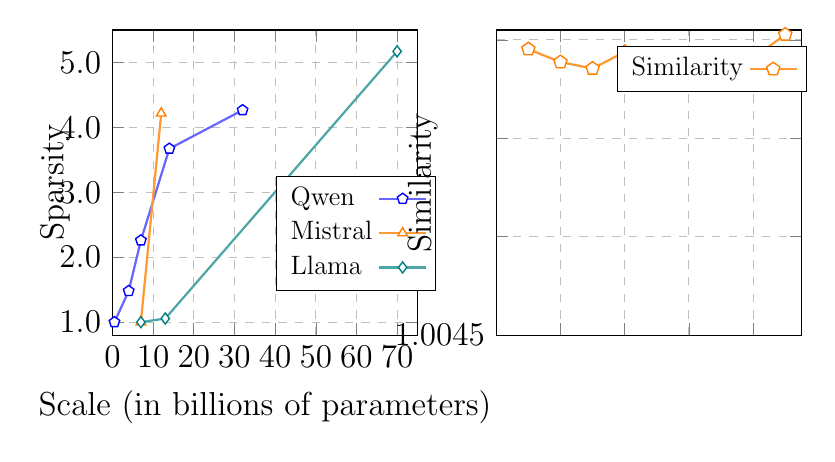
\begin{tikzpicture} % 开始绘图
    \large
    % 设置第一个图表的样式
    \begin{axis}[
     at={(0,0)},
      name=plot1, % 图表名称
      ymajorgrids, % 主要网格线
      xmajorgrids, % 主要网格线
      grid style=dashed, % 网格线样式
      width=.45\textwidth, % 图表宽度
      height=.45\textwidth, % 图表高度
      legend style={at={(0.75,0.2)}, anchor=south west}, % 图例位置
      xlabel={Scale (in billions of parameters)}, % X轴标签
      ylabel={Sparsity}, % Y轴标签
      ylabel style={yshift=-1em}, % Y轴标签偏移
      xlabel style={yshift=0.0em}, % X轴标签偏移
      yticklabel style={/pgf/number format/precision=1, /pgf/number format/fixed zerofill}, % Y轴刻度标签格式
      ymin=0.8, ymax=5.5, % Y轴范围
      ytick={1,2,3,4,5}, % Y轴刻度
      xmin=0, xmax=75, % X轴范围
      xtick={0,10,20,30,40,50,60,70}, % X轴刻度
      legend style={yshift=-6pt, xshift=-2em, legend plot pos=right, font={\large}, cells={anchor=west}} % 图例样式
    ]

    % 绘制第一个图表的数据系列
    \addplot[blue!60,mark=pentagon*,mark size=2pt,thick,mark options={fill=white,draw=blue,line width=0.5pt}] 
    coordinates {(0.5,1) (4,1.479851452) (7,2.259327441) (14,3.672399561) (32,4.265417883)};
    \addlegendentry{\scalebox{.8}{Qwen}} % 图例条目

    \addplot[orange!80,mark=triangle*,mark size=2pt,thick,mark options={fill=white,draw=orange,line width=0.5pt}] 
    coordinates {(7,1) (12,4.218270426)};
    \addlegendentry{\scalebox{.8}{Mistral}} % 图例条目

    \addplot[teal!70,mark=diamond*,mark size=2pt,thick,mark options={fill=white,draw=teal,line width=0.5pt}] 
    coordinates {(7,1) (13,1.055636607) (70,5.171299311)};
    \addlegendentry{\scalebox{.8}{Llama}} % 图例条目

    \end{axis}

    % 设置第二个图表的样式
    \begin{axis}[
      at={(0,0)},
      name=plot2,
      at={(plot1.east)}, % 第二个图表位置相对于第一个图表
      anchor=west,
      xshift=1cm, % X轴偏移
      ymajorgrids,
      xmajorgrids,
      grid style=dashed,
      width=.45\textwidth,
      height=.45\textwidth,
      legend style={at={(0.61,0.85)}, anchor=south west},
      xlabel={}, % X轴标签
      ylabel={Similarity}, % Y轴标签
      ylabel style={yshift=-2.0em},
      xlabel style={yshift=0.0em},
      yticklabel style={/pgf/number format/precision=1, /pgf/number format/fixed zerofill},
      ymin=1, ymax=1.0062, % Y轴范围
      %ytick={0.9975,1.00,1.003,1.006,1.009,1.012}, % Y轴刻度
      yticklabels={,1.0045,,,,,}, % Y轴刻度标签
      xmin=0, xmax=9.5, % X轴范围
      xtick={},
      xticklabels={},
      legend style={yshift=-6pt, xshift=-2em, legend plot pos=right, font={\large}, cells={anchor=west}} % 图例样式
    ]

    % 绘制第二个图表的数据系列
    \addplot[orange!80,mark=pentagon*,mark size=2.5pt,thick,mark options={fill=white,draw=orange,line width=0.5pt}]
    coordinates {(1,1.005810968) (2,1.005548433) (3,1.005417148) (4,1.005755459) (5,1.005575278) (6,1.005482516) (7,1.005250273) (8,1.005630629) (9,1.006107432)};
    \addlegendentry{\scalebox{.8}{Similarity}} % 图例条目
    



    \end{axis}

  \end{tikzpicture}
  \caption{wwwwwww} % 图形标题
  \label{fig:data-comparison} % 标签
\end{figure}

\end{document}